\begin{enumerate}
\item The constraints are as follows:
  \begin{align*}
    x_1 -x_2 &\geq -2.5, &(1)\\
    3x_1 + 4x_2 &\leq 24, & (2) \\
    x_1 - x_2 &\leq 4, & (3) \\
    x_1 &\geq 0, & (4) \\
    x_2 &\geq 0. & (5)
  \end{align*}

\item  We now write the problem in  standard form. We include the
  following  slack variables to the inequality constraints to obtain
  equality constraints:
  \begin{itemize}
  \item $x_3$ for constraint (1),
  \item $x_4$ for constraint (2), and,
  \item $x_5$ for constraint (3).
  \end{itemize}
  Moreover, a maximization problem whose objective function is $f(x)$ is equivalent to a minimization problem
  whose objective function is $-f(x)$. Then we obtain the following problem.

  \[
    \min_{x \in \R^5}  -x_1  -x_2
    \]
    subject to
  \[
  \begin{array}{rrrrrr cl r}
     x_1 &  - x_2 &  - x_3 & & & &= & -2.5, & \\
     3 x_1 & +4 x_2 & &  + x_4 & & &= & 24, & \\
     x_1 & - x_2 & & &  + x_5 & &= & 4, & \\
     & & & & &  x_i & \geq & 0, &  i = 1,\ldots, 5.
  \end{array}
  \]

  The number of equality constraints is $m=3$ and the number of decision variables is $n=5$.
  The matrix  $A\in\R^{m\times n}$ and the vectors $b\in\R^{m}$ and $c\in\R^{n}$ are given by
  \[
  A =
  \begin{pmatrix}
    1 & -1 & -1 & 0 & 0 \\
    3 & 4 & 0 & 1 & 0\\
    1 & -1 & 0 & 0 & 1
  \end{pmatrix}, \qquad
  b = \begin{pmatrix}
    -2.5 \\
    24 \\
    4
  \end{pmatrix}, \qquad
  c = \begin{pmatrix}
    -1 \\
    -1 \\
    0 \\
    0 \\
    0
  \end{pmatrix}.
  \]

\item  Each basic solution is obtained by selecting $m=3$ variables out of $n=5$ to be in the basis.
  The $n-m=2$ non basic variables equal to 0.
  There is a total of 10 possible selections of basic variables. We
  detail the  computation of some of them.
  \begin{itemize}
  \item Basic solution with $x_1$, $x_2$ and $x_3$ in the basis

    ($j_1=1$, $j_2=2$, $j_3=3$).
    $$B=
    \begin{pmatrix}
      1 & -1 & -1 \\
      3 & 4 & 0 \\
      1 & -1 & 0
    \end{pmatrix};
    \quad
    B^{-1}=
    \begin{pmatrix}
      0 & 1/7 & 4/7 \\
      0 & 1/7 & -3/7 \\
      -1 & 0 & 1
    \end{pmatrix};
    $$

    $$
    x_B = B^{-1}b=
    \begin{pmatrix}
      40/7  \\
      12/7 \\
      13/7
    \end{pmatrix};
    \quad
    x=
    \begin{pmatrix}
      40/7  \\
      12/7 \\
      13/7  \\
      0\\
      0
    \end{pmatrix}.
    $$
    This basic solution is feasible since $ B^{-1}b  \geq 0$. It corresponds to point C in Figure  \ref{fig:a18-bassol}
    which is the intersection of constraints (2) and (3). Note that
    activating constraints (2) and (3) in the original problem is
    equivalent to setting to zero the slack variables $x_4$ and $x_5$ in the
    problem in standard form. These are the non basic variables that
    are set to zero.


  \item Basic solution with $x_1$, $x_2$ and $x_5$ in the basis

    ($j_1=1$, $j_2=2$, $j_3=5$).
    $$B=
    \begin{pmatrix}
      1 & -1 & 0 \\
      3 & 4 & 0 \\
      1 & -1 & 1
    \end{pmatrix};
    \quad
    B^{-1}=
    \begin{pmatrix}
      4/7 & 1/7 & 0 \\
      -3/7 & 1/7 & 0 \\
      -1 & 0 & 1
    \end{pmatrix};
    $$

    $$
    x_B = B^{-1}b=
    \begin{pmatrix}
      2  \\
      4.5 \\
      6.5
    \end{pmatrix};
    \quad
    x=
    \begin{pmatrix}
      2  \\
      4.5 \\
      0  \\
      0\\
      6.5
    \end{pmatrix}.
    $$
    This basic solution is feasible as $ B^{-1}b  \geq 0$. It corresponds to vertex H in Figure  \ref{fig:a18-bassol}
    which is the intersection of constraints (1) and (2). Note that
    activating constraints (1) and (2) in the original problem is
    equivalent to setting to zero the slack variables $x_3$ and $x_4$ in the
    problem in standard form. These are the non basic variables that
    are set to zero.

  \item  Basic solution with $x_1$, $x_3$ and $x_5$ in the basis

    ($j_1=1$, $j_2=3$, $j_3=5$).
    $$B=
    \begin{pmatrix}
      1 & -1 & 0 \\
      3 & 0 & 0 \\
      1 & 0 & 1
    \end{pmatrix};
    \quad
    B^{-1}=
    \begin{pmatrix}
      0 & 1/3 & 0 \\
      -1 & 1/3 & 0 \\
      0 & -1/3 & 1
    \end{pmatrix};
    $$

    $$
    x_B = B^{-1}b=
    \begin{pmatrix}
      8  \\
      10.5 \\
      -4
    \end{pmatrix};
    \quad
    x=
    \begin{pmatrix}
      8  \\
      0 \\
      10.5\\
      0\\
      -4
    \end{pmatrix}.
    $$
    This basic solution is not feasible since $ B^{-1}b  \ngeq 0$. It corresponds to vertex E in Figure  \ref{fig:a18-bassol}
    which is the intersection of constraints (2) and (5). Note that
    activating constraints (2) and (5) in the original problem is
    equivalent to setting to zero the slack variable $x_4$ and the variable $x_2$ in the
    problem in standard form. These are the non basic variables that
    are set to zero.
  \end{itemize}


  The following table gives all the basic solutions. Each basic solution is obtained by fixing
  $n-m=2$ non basic variables, which equal  0, and calculating the other variables using
  $x_B= B^{-1}b$.

  \begin{center}
    %\resizebox{\textwidth}{6cm}{
    \begin{tabular}{|c||c|c||c|c|c|c|c||c||c|}
      \hline
      \text{Point} & $x_1$ & $x_2$ & $x_3$ & $x_4$ & $x_5$ & Feasible? \\
      \hline
      A & 0 & 6 & -3.5 & 0 & 10   & no \\
      B & 0 & 0 & 2.5 & 24 & 4  &  yes \\
      C & 40/7 & 12/7 & 13/7 & 0 & 0 & yes \\
      D & 4 & 0 & 6.5 & 12 & 0  & yes \\
      E & 8 & 0 & 10.5 & 0 & -4  & no  \\
      F & 0 & -4 & 6.5 &	 40 &  0 & no \\
      G & 0 & 2.5 &  0 & 14 & 6.5  & yes\\
      H & 2 & 4.5 & 0 &	0 & 6.5  & yes \\
      I & -2.5 & 0 & 0 & 31.5 & 6.5 &  no \\
      -- & -- & -- & 0 & --  & 0&    \\
      \hline
    \end{tabular}
    %	}
  \end{center}

  Note: It is impossible to have the case $ x_3 = x_5 = 0 $. In other words, $x_3$ and $x_5$ can't be non basic variables in the same time.
  Indeed, in this case the basic matrix is
  $$B=(A_1,A_2,A_4)=
  \begin{pmatrix}
    1 & -1 & 0 \\
    3 & 4 & 1 \\
    1 & -1 & 0
  \end{pmatrix}
  $$ which is a singular matrix. Therefore, there is no corresponding
  basic solution.  In fact, having $ x_3 = x_5 = 0$ means that
  constraints (1) and (3) are active at  the same time, which is
  impossible since these two constraints are parallel.  This case is
  represented with dashes in the table.


  \begin{itemize}
  \item In Figure  \ref{fig:a18-bassol}, the basic solutions are given with the same letters as on the table above: from A to I.
    They correspond to the intersections of the constraints.


    \begin{figure}[htb]
      \begin{center}
	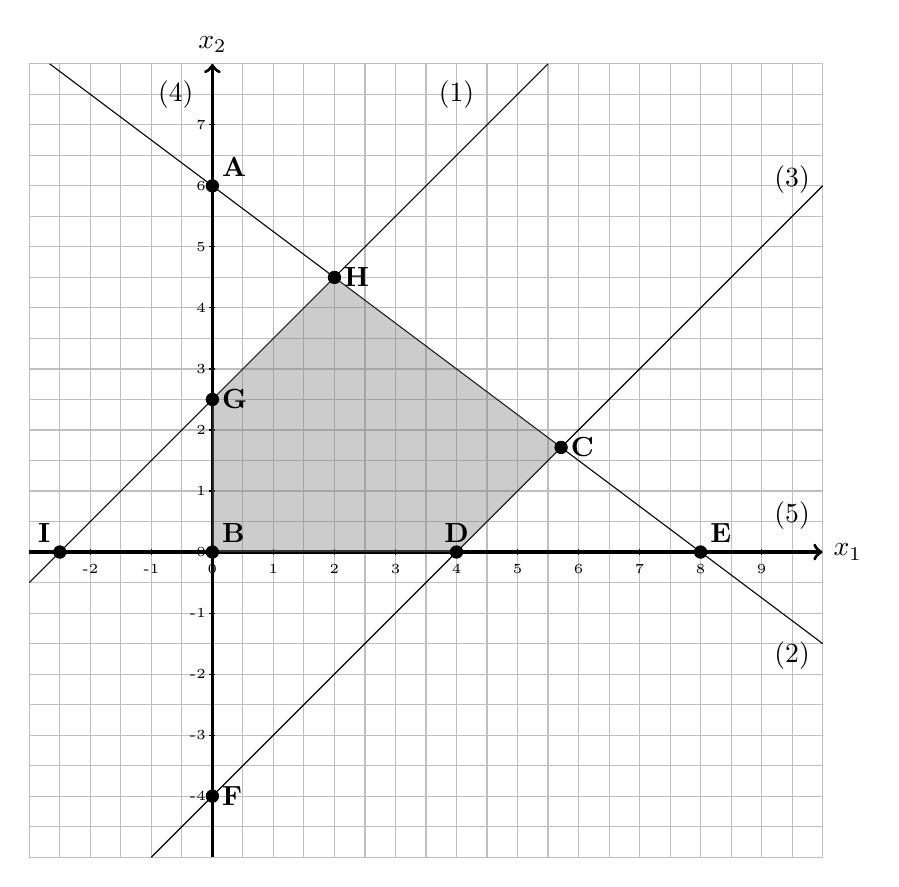
\begin{tikzpicture}[scale=0.775]
	  \draw[gray!50, thin, step=0.5] (-3,-5) grid (10,8);
    	  \draw[very thick,->] (-3,0) coordinate(x1) -- (10,0) coordinate(x2) node[right] {$x_1$};
    	  \draw[very thick,->] (0,-5) coordinate(y1) -- (0,8) coordinate(y2) node[above] {$x_2$};
	  \foreach \x in {-2,...,9} \draw (\x,0.05) -- (\x,-0.05) node[below] {\tiny\x};
	  \foreach \y in {-4,...,7} \draw (-0.05,\y) -- (0.05,\y) node[left] {\tiny\y};


	  \draw (-3,-0.5)--(5.5,8);
	  \draw (-8/3,8)--(10,-1.5);
	  \draw (-1,-5)--(10,6);



	  \node at (9.5,-1.7){(2)};
	  \node at (9.5, 6.1){(3)};
	  \node at (-0.6,7.5){(4)};
	  \node at (9.5,0.6){(5)};
	  \node at (4,7.5){(1)};



	  \fill[gray,opacity=0.4] (0,0) -- (0,2.5) -- (2,4.5) -- (40/7,12/7)--(4,0)  --cycle;



	  \draw [draw = black,fill=black] (0,6) circle (0.1) node[anchor=south west] {\textbf{A}};

	  \draw [draw = black,fill=black] (0,0) circle (0.1) node[anchor=south west] {\textbf{B}};

	  \draw [draw = black,fill=black] (40/7,12/7) circle (0.1) node[anchor=west] {\textbf{C}};

	  \draw [draw = black,fill=black] (4,0) circle (0.1) node[anchor=south] {\textbf{D}};

	  \draw [draw = black,fill=black] (8,0) circle (0.1) node[anchor=south west] {\textbf{E}};

	  \draw [draw = black,fill=black] (0,-4) circle (0.1) node[anchor=west] {\textbf{F}};

	  \draw [draw = black,fill=black] (0,2.5) circle (0.1) node[anchor=west] {\textbf{G}};

	  \draw [draw = black,fill=black] (2,4.5) circle (0.1) node[anchor=west] {\textbf{H}};

	  \draw [draw = black,fill=black] (-2.5,0) circle (0.1) node[anchor= south east] {\textbf{I}};


	\end{tikzpicture}
	\caption{\label{fig:a18-bassol}Basic solutions}
      \end{center}
    \end{figure}


  \item A solution is feasible if it satisfies all the constraints of
    the problem. In order to calculate the basic solutions, we used
    the formula $x_B= \nolinebreak B^{-1}b$.  The non negativity
    constraints still need to be satisfied. The feasible solutions
    satisfies $$ x_i \geq 0, \quad \forall i \in {1,\ldots,5}.$$
    Therefore, the feasible basic solutions corresponds to the
    following points:
    \begin{center}
      B(0, 0), C(40/7, 12/7), D(4, 0), G(0, 2.5) and H(2, 4.5),
    \end{center}
    that happen to be the vertices of the polyhedron.


  \end{itemize}


\item When considering the problem in standard form,
  the point (3, 2) corresponds to the
  point ($ x_1 $, $ x_2 $, $ x_3 $,
  $ x_4 $, $ x_5 $) = (3, 2, 3.5, 7, 3). This is a feasible solution because all the constraints are
  satisfied.

  However,  in a basic solution at least $n$ constraints must be active.
  In standard form, $n=5$. There are $m=3$ equality constraints that are active.
  Therefore, at least two variables (the non basic variables) should be zero at a basic solution.
  It is not the case for point (3, 2), so it is not a basic solution.


\item Given a feasible point of the polyhedron, it is possible to analyze if a
  direction is feasible by checking the following two conditions:

  \begin{itemize}
  \item $Ad=0$ and
  \item $d_i \geq 0$ when $x_i=0$,
  \end{itemize}
  where

  \[
  A =
  \begin{pmatrix}
    1 & -1 & -1 & 0 & 0 \\
    3 & 4 & 0 & 1 & 0\\
    1 & -1 & 0 & 0 & 1
  \end{pmatrix}, \qquad
  x = \begin{pmatrix}
    x_1 \\
    x_2 \\
    x_3\\
    x_4\\
    x_5
  \end{pmatrix}, \qquad
  d = \begin{pmatrix}
    d_1 \\
    d_2 \\
    d_3 \\
    d_4 \\
    d_5
  \end{pmatrix}.
  \]


  We verify if these conditions are satisfied for the case  $x= \begin{pmatrix}
    4 \\
    0
  \end{pmatrix}$
  and
  $d=  \begin{pmatrix}
    1 \\
    1
  \end{pmatrix}.$

  We first need to compute the values of the slack variables $x_3$,  $x_4$
  and $x_5$. We obtain $x_3 = 6.5$,  $x_4= 12$ and $x_5=0$. Therefore, we have

  $$
  x = \begin{pmatrix}
    4 \\
    0 \\
    6.5\\
    12\\
    0
  \end{pmatrix}.
  $$

  In order to satisfy the first condition, we must have

  \[
  A d =
  \begin{pmatrix}
    1 & -1 & -1 & 0 & 0 \\
    3 & 4 & 0 & 1 & 0\\
    1 & -1 & 0 & 0 & 1
  \end{pmatrix}
  \begin{pmatrix}
    1 \\
    1 \\
    d_3\\
    d_4\\
    d_5
  \end{pmatrix} =
  \begin{pmatrix}
    - d_3 \\
    7+d_4 \\
    d_5
  \end{pmatrix}=
  \begin{pmatrix}
    0 \\
    0 \\
    0
  \end{pmatrix}.
  \]

  which is verified by setting $d_3 = 0$, $d_4 = -7$ and  $d_5 = 0$. Therefore, %$d_4 = −7$ and $d_5=0$. Therefore,

  $$
  d = \begin{pmatrix}
    1 \\
    1 \\
    0 \\
    -7 \\
    0
  \end{pmatrix}.
  $$

  satisfies the first condition. For the second, we need to look at the
  entries 2 and 5 of $d$ since $ x_2 = x_5 = 0$. As both entries are non negative,
  we conclude that the direction is feasible at the given point.

\end{enumerate}
